{
\section{Definition of the Brownian web}
\label{sec:brownian-web-definition}

The Brownian web is the continuum scaling limit of a system of
independent-coalescing random walks (see
\cite{tsirelson-lecture-course}).  Constructing the
continuum version raises several technical difficulties addressed in
\cite{fontes-et-al},\cite{norris-turner},\cite{toth-werner}.
Nonetheless, all the
constructions share the following property, which we use as a
definition:

\newcommand{\simplex}{\mathcal{S}}

  Denote $\simplex=\{(s, t) \in \R^2 : s \le t\}$.
  A Brownian web on a probability space $\Omega$ is a (jointly)
  measurable mapping $\webnoargs : \Omega \cross \simplex \cross \R
  \to \R$, $(\omega, (s, t), x) \mapsto \web{s}{t}{x}$ (suppressing
  $\omega$ in the notation) such that for every finite collection of
  starting points $(s_1, x_1),(s_2, x_2),...,(s_n, x_n)$, the
  collection of processes $\web{s_1} {\cdot}{x_1},
  \web{s_2}{\cdot}{x_2},...,\web{s_n}{\cdot}{x_n}$
  forms a system of $n$ independent-coalescing Brownian motions.

  \newcommand{\bm}[1]{X^{#1}}

  A system of $n$ independent-coalescing Brownian motions is a finite
  collection of stochastic processes $(\bm{1}, \bm{2},...,\bm{n})$ such that
  each $\bm{i}$ starts at some point $x_i$ at some time $s_i$, and $(\bm{1},
  \bm{2},...,\bm{n})$ are independent until the first time $T$ at which
  $\bm{i}(T)=\bm{j}(T)$ for some $i\neq j$. From this time onwards $\bm{i}(T)$
  and $\bm{j}(T)$ coalesce and continue with the rest of the $\bm{k}$ (for
  $k\neq i,j$) as a system of $n-1$ independent-coalescing Brownian motions.
  Several trajectories of a Brownian web can be seen in Figure
  \ref{fig:bw-trajectories}.

\begin{figure}
   \centering
   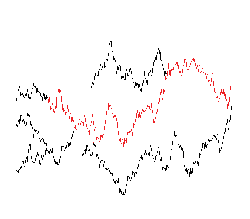
\includegraphics[scale=2]{sometraj.eps}
   \caption{Some trajectories of the Brownian web. A particular trajectory is marked.}
  \label{fig:bw-trajectories}
\end{figure}
}
